\documentclass[aspectratio = 169]{chariteBeamer}
\usepackage[english]{babel} %% english
\usepackage[utf8]{inputenc}
\usepackage[T1]{fontenc}
\usepackage{hyperref}
\usepackage{blkarray}
\tikzset{>=latex}
\usepackage[edges]{forest}
\usetikzlibrary{positioning}
\usepackage{biostat}
\setbeamertemplate{caption}[numbered]
\let\qed\relax
\forestset{declare toks={elo}{}}
\graphicspath{{figures/}}
%% ================================================================== %% 

\author[L. Mödl, M. Becher, E. Sprünken]{Lukas Mödl, Matthias Becher, Erin Sprünken} 
\title{Day 4 -- Control Flow} 
\date[]{Updated: \today}
\place{R-Course}
\email{biometrie-rkurs@charite.de}

%% ================================================================== %% 

\hyphenation{Sam-ples}
\begin{document}

\begin{frame}[plain]
    \titlepage%
\end{frame}

\frame{\tableofcontents}


\section{Programming I: Conditions}

\begin{frame}[fragile]{if-statement}
    If we want to execute a block of code dependent on a certain value, we choose an if-statement. If-statements define such code-blocks, that will only be executed if a certain user-defined condition is true.\bigskip \\
    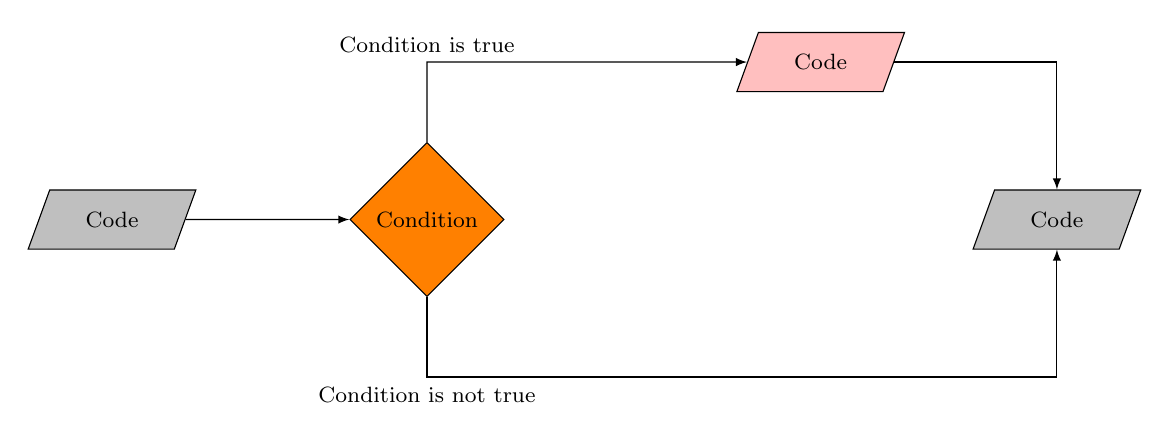
\begin{tikzpicture}
      \node[draw, trapezium, trapezium left angle=70, trapezium right angle=-70, minimum height=0.75cm, fill=gray!50!white] (n0) {\footnotesize Code};
      \node[draw, diamond, right of=n0, node distance=4cm, fill=orange] (n1) { \footnotesize Condition};
      \coordinate[below of=n1, node distance=2cm] (aux1);
      \coordinate[above of=n1, node distance=2cm] (aux2);
      \node[draw, trapezium, trapezium left angle=70, trapezium right angle=-70, right of=aux2, node distance=5cm, minimum height=0.75cm,fill=pink] (n2) { \footnotesize Code};
      \node[draw, trapezium, trapezium left angle=70, trapezium right angle=-70, right of=n1, node distance=8cm, minimum height=0.75cm, fill=gray!50!white] (n3) {\footnotesize Code};
      \draw[->] (n0) to (n1);
      \draw[->] (n1.north) to (aux2) node[anchor=south]{\footnotesize Condition is true} to (n2);
      \draw[->] (n2) -| (n3);
      \draw[->] (n1.south) to (aux1) node[anchor=north]{\footnotesize Condition is not true} -| (n3);
    \end{tikzpicture}
\end{frame}

\begin{frame}[fragile]{Example if-statement}
  To understand the idea, we want to assign the value \verb+2+ to \verb+x+. Dependent on the value of \verb+x+ we want to print an output. \bigskip \\
      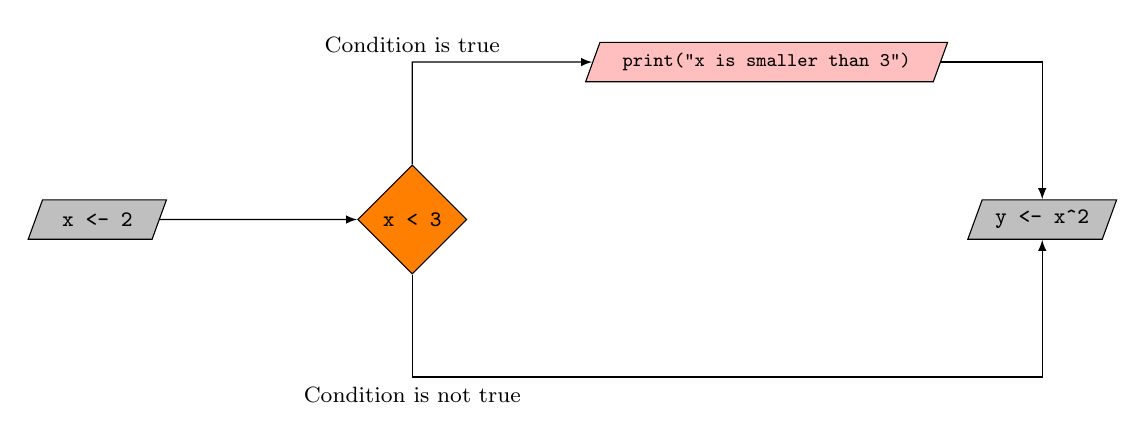
\begin{tikzpicture}
      \node[draw, trapezium, trapezium left angle=70, trapezium right angle=-70, minimum height=0.5cm, fill=gray!50!white] (n0) {\footnotesize\verb+x <- 2+};
      \node[draw, diamond, right of=n0, node distance=4cm, fill=orange] (n1) { \footnotesize \verb+x < 3+};
      \coordinate[below of=n1, node distance=2cm] (aux1);
      \coordinate[above of=n1, node distance=2cm] (aux2);
      \node[draw, trapezium, trapezium left angle=70, trapezium right angle=-70, right of=aux2, node distance=4.5cm, minimum height=0.5cm,fill=pink] (n2) {\scriptsize\verb+print("x is smaller than 3")+};
      \node[draw, trapezium, trapezium left angle=70, trapezium right angle=-70, right of=n1, node distance=8cm, minimum height=0.5cm, fill=gray!50!white] (n3) {\footnotesize\verb+y <- x^2+};
      \draw[->] (n0) (n0) to (n1);
      \draw[->] (n1.north) to (aux2) node[anchor=south]{\footnotesize Condition is true} to (n2);
      \draw[->] (n2) -| (n3);
      \draw[->] (n1.south) to (aux1) node[anchor=north]{\footnotesize Condition is not true} -| (n3);
    \end{tikzpicture}
\end{frame}

\begin{frame}[fragile]{Example if-statement}
  To understand the idea, we want to assign the value \verb+2+ to \verb+x+. Dependent on the value of \verb+x+ we want to print an output. \bigskip \\
  \begin{center}
  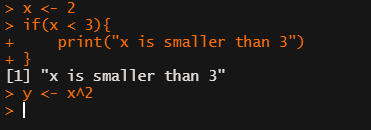
\includegraphics[]{if1.png}
  \end{center}
\end{frame}

\begin{frame}[fragile]{if-else-statement}
  Sometimes, we don't want to test for only one condition but rather have an either this or that situation. In that case, we use the if-else-statement. \bigskip \\  
    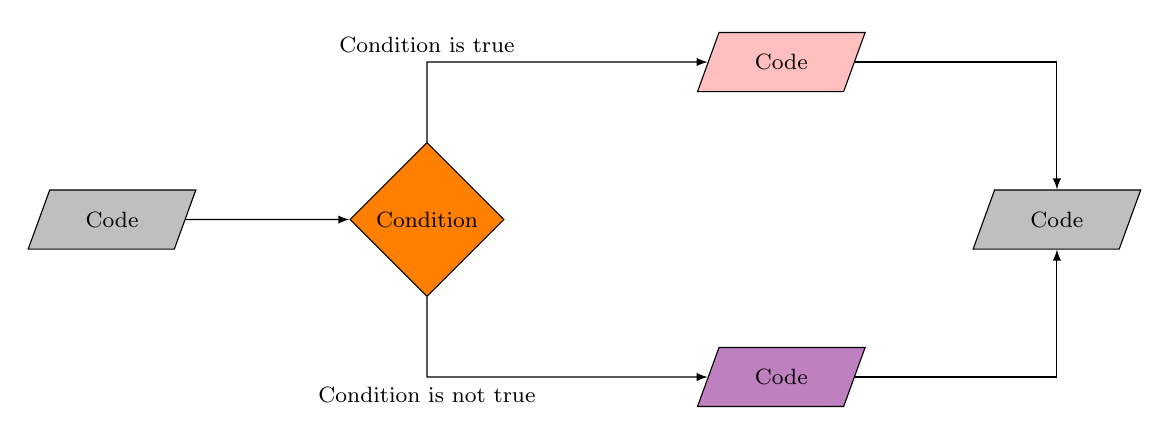
\begin{tikzpicture}
      \node[draw, trapezium, trapezium left angle=70, trapezium right angle=-70, minimum height=0.75cm, fill=gray!50!white] (n0) {\footnotesize Code};
      \node[draw, diamond, right of=n0, node distance=4cm, fill=orange] (n1) { \footnotesize Condition};
      \coordinate[below of=n1, node distance=2cm] (aux1);
      \coordinate[above of=n1, node distance=2cm] (aux2);
      \node[draw, trapezium, trapezium left angle=70, trapezium right angle=-70, right of=aux2, node distance=4.5cm, minimum height=0.75cm,fill=pink] (n21) { \footnotesize Code};
      \node[draw, trapezium, trapezium left angle=70, trapezium right angle=-70, right of=aux1, node distance=4.5cm, minimum height=0.75cm,fill=violet!50!white] (n22) { \footnotesize Code};
      \node[draw, trapezium, trapezium left angle=70, trapezium right angle=-70, right of=n1, node distance=8cm, minimum height=0.75cm, fill=gray!50!white] (n3) {\footnotesize Code};
      \draw[->] (n0) to (n1);
      \draw[->] (n1.north) to (aux2) node[anchor=south]{\footnotesize Condition is true} to (n21);
      \draw[->] (n22) -| (n3);
      \draw[->] (n21) -| (n3);
      \draw[->] (n1.south) to (aux1) node[anchor=north]{\footnotesize Condition is not true} to (n22);
    \end{tikzpicture}
\end{frame}

\begin{frame}[fragile]{Example if-else-statement}
    To understand this concept, we will modify our former example. \bigskip \\
    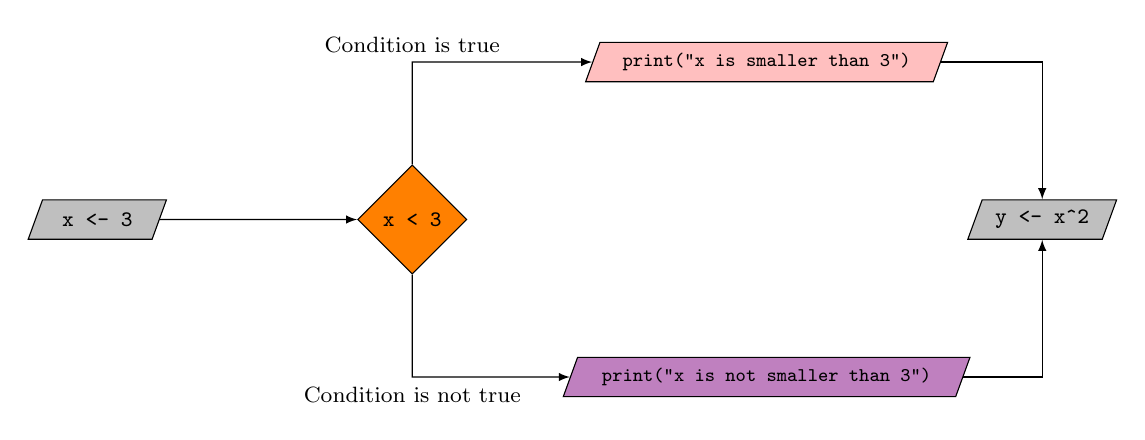
\begin{tikzpicture}
      \node[draw, trapezium, trapezium left angle=70, trapezium right angle=-70, minimum height=0.5cm, fill=gray!50!white] (n0) {\footnotesize\verb+x <- 3+};
      \node[draw, diamond, right of=n0, node distance=4cm, fill=orange] (n1) { \footnotesize \verb+x < 3+};
      \coordinate[below of=n1, node distance=2cm] (aux1);
      \coordinate[above of=n1, node distance=2cm] (aux2);
      \node[draw, trapezium, trapezium left angle=70, trapezium right angle=-70, right of=aux2, node distance=4.5cm, minimum height=0.5cm,fill=pink] (n21) { \scriptsize \verb+print("x is smaller than 3")+};
      \node[draw, trapezium, trapezium left angle=70, trapezium right angle=-70, right of=aux1, node distance=4.5cm, minimum height=0.5cm,fill=violet!50!white] (n22) { \scriptsize \verb+print("x is not smaller than 3")+};
      \node[draw, trapezium, trapezium left angle=70, trapezium right angle=-70, right of=n1, node distance=8cm, minimum height=0.5cm, fill=gray!50!white] (n3) {\footnotesize \verb+y <- x^2+};
      \draw[->] (n0) to (n1);
      \draw[->] (n1.north) to (aux2) node[anchor=south]{\footnotesize Condition is true} to (n21);
      \draw[->] (n22) -| (n3);
      \draw[->] (n21) -| (n3);
      \draw[->] (n1.south) to (aux1) node[anchor=north]{\footnotesize Condition is not true} to (n22);
    \end{tikzpicture}
\end{frame}

\begin{frame}[fragile]{Example if-else-statement}
    To understand this concept, we will modify our former example. \bigskip\\
  \begin{center}
  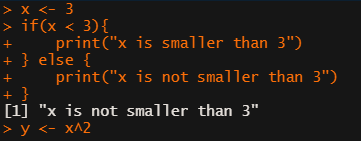
\includegraphics[]{if2.png}
  \end{center}
\end{frame}

\begin{frame}[fragile]{Remarks to the if-else-statement}
  \begin{itemize}
    \item Using the brackets \verb+{+ and \verb+}+ is essential!
    \item Only logical statements are allowed as a condition
    \item Sometimes, nested statements and conditions are necessary
    \item Indentation is improving the readability of a code!
  \end{itemize}
\end{frame}

\section{Programming II: Loops}

\begin{frame}[fragile]{for-Loop}
    An important loop in \textsf R is the for-loop. For-loops execute a block of code as often as a certain index variable in an index set (a vector or a list) exists. We construct this by the keyword \verb+for()+ followed by a block of code in curly brackets. The round parentheses are used to determine the index variable and index set. \bigskip \\
    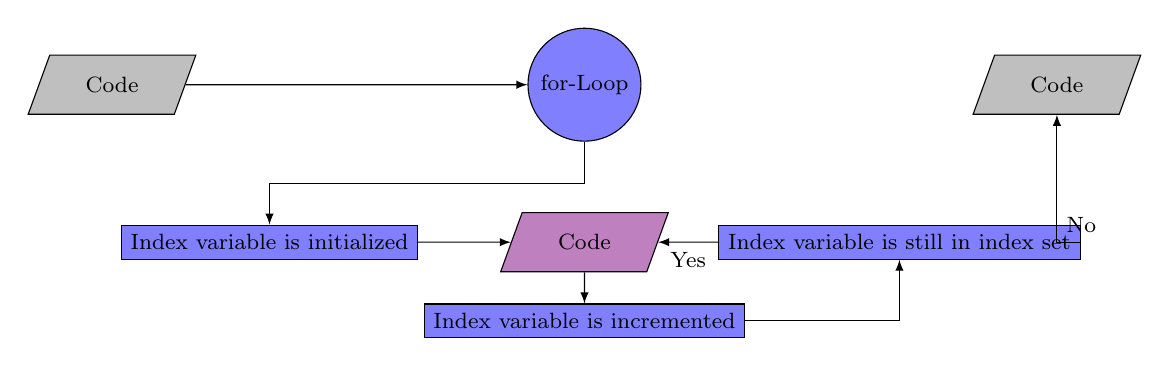
\begin{tikzpicture}
      \node[draw, trapezium, trapezium left angle=70, trapezium right angle=-70, minimum height=0.75cm, fill=gray!50!white] (n0) {\footnotesize Code};
      \node[draw, trapezium, trapezium left angle=70, trapezium right angle=-70, right of=n0, node distance=12cm, minimum height=0.75cm, fill=gray!50!white] (nx) {\footnotesize Code};
      \coordinate[below of=n0, node distance=2cm] (aux1);
      \coordinate[below of=nx, node distance=2cm] (aux2);
      \node[draw, circle, right of=n0, node distance=6cm, fill=blue!50!white] (n1) { \footnotesize for-\newline\footnotesize Loop};
      \node[rectangle, draw, right of=aux1, node distance=2cm,fill=blue!50!white] (n2) {\footnotesize Index variable is initialized};
      \node[draw, trapezium, trapezium left angle=70, trapezium right angle=-70, below of=n1, node distance=2cm, minimum height=0.75cm,fill=violet!50!white] (n3) { \footnotesize Code};
      \node[rectangle, draw, below of=n3, node distance=1cm,fill=blue!50!white] (n4) {\footnotesize Index variable is incremented};
      \node[rectangle, draw, right of=n3, node distance=4cm,fill=blue!50!white] (n5) {\footnotesize Index variable is still in index set};
      \draw[->] (n0) to (n1);
      %\draw[->] (n1) to (nx);
      \coordinate[below of=n1, node distance=1.25cm] (aux3);
      \draw[->] (n1.south) -- (aux3) -| (n2.north);
      \draw[->] (n2) to (n3);
      \draw[->] (n5) to node[anchor=north]{\footnotesize Yes} (n3);
      \draw[<-] (n5) |- (n4);
      \draw[->] (n3) to (n4);
      \draw[->] (n5.east) -| node[anchor=south west]{\footnotesize No} (nx.south);
    \end{tikzpicture}
\end{frame}

\begin{frame}[fragile]{Example for-Loop}
  This example emphasizes the for-loop. Here, \verb+I+ is the index set and \verb+i+ the index variable. \bigskip\\
    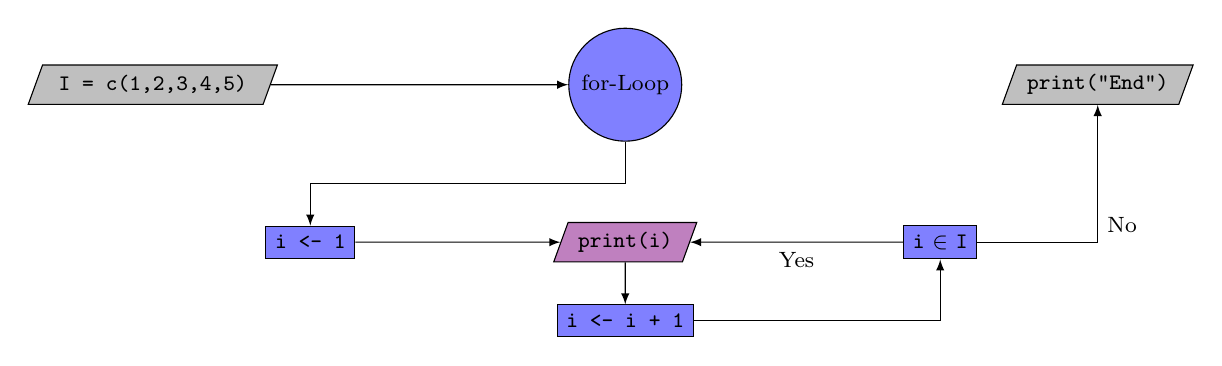
\begin{tikzpicture}
      \node[draw, trapezium, trapezium left angle=70, trapezium right angle=-70, minimum height=0.5cm, fill=gray!50!white] (n0) {\footnotesize \verb+I = c(1,2,3,4,5)+};
      \node[draw, trapezium, trapezium left angle=70, trapezium right angle=-70, right of=n0, node distance=12cm, minimum height=0.5cm, fill=gray!50!white] (nx) {\footnotesize\verb+print("End")+};
      \coordinate[below of=n0, node distance=2cm] (aux1);
      \coordinate[below of=nx, node distance=2cm] (aux2);
      \node[draw, circle, right of=n0, node distance=6cm, fill=blue!50!white] (n1) { \footnotesize for-\newline\footnotesize Loop};
      \node[rectangle, draw, right of=aux1, node distance=2cm,fill=blue!50!white] (n2) {\footnotesize\verb+i <- 1+};
      \node[draw, trapezium, trapezium left angle=70, trapezium right angle=-70, below of=n1, node distance=2cm, minimum height=0.5cm,fill=violet!50!white] (n3) { \footnotesize \verb+print(i)+};
      \node[rectangle, draw, below of=n3, node distance=1cm,fill=blue!50!white] (n4) {\footnotesize \verb.i <- i + 1.};
      \node[rectangle, draw, right of=n3, node distance=4cm,fill=blue!50!white] (n5) {\footnotesize \verb+i+ $\in$ \verb+I+};
      \draw[->] (n0) to (n1);
      %\draw[->] (n1) to (nx);
      \coordinate[below of=n1, node distance=1.25cm] (aux3);
      \draw[->] (n1.south) -- (aux3) -| (n2.north);
      \draw[->] (n2) to (n3);
      \draw[<-] (n3) to node[anchor=north]{\footnotesize Yes} (n5);
      \draw[<-] (n5) |- (n4);
      \draw[->] (n3) to (n4);
      \draw[->] (n5.east) -| node[anchor=south west]{\footnotesize No} (nx.south);
    \end{tikzpicture}
\end{frame}

\begin{frame}[fragile]{Example for-Loop}
  This example emphasizes the for-loop. Here, \verb+I+ is the index set and \verb+i+ the index variable. \bigskip\\
  \begin{centering}
  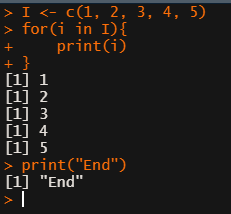
\includegraphics[]{for1.png}
  \end{centering}
\end{frame}

\subsection*{while-Loop}

\begin{frame}[fragile]{while-Loop}
	Another elementary loop is the while-loop. Contrary to the for-loop it executes code \textit{while} a certain condition is true. It is constructed using the keyword \verb+while()+ followed by a block of code in curly brackets. Within the round parentheses the condition is given. \bigskip \\
   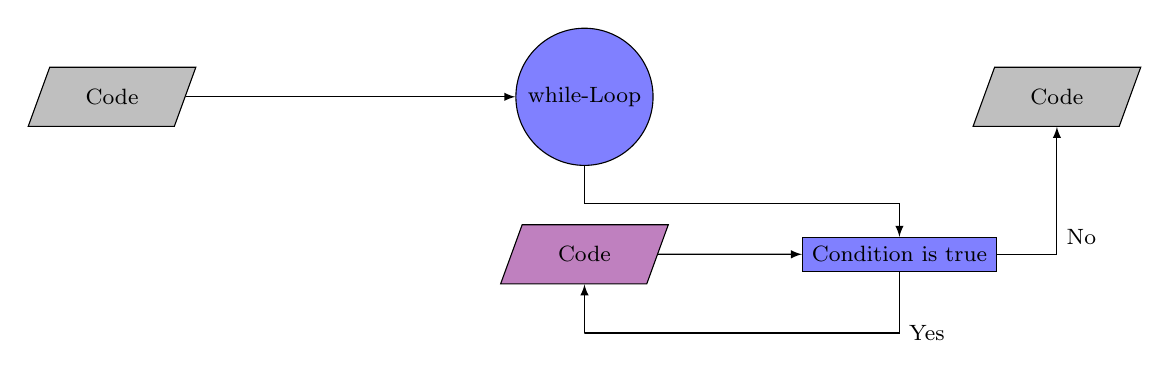
\begin{tikzpicture}
      \node[draw, trapezium, trapezium left angle=70, trapezium right angle=-70, minimum height=0.75cm, fill=gray!50!white] (n0) {\footnotesize Code};
      \node[draw, trapezium, trapezium left angle=70, trapezium right angle=-70, right of=n0, node distance=12cm, minimum height=0.75cm, fill=gray!50!white] (nx) {\footnotesize Code};
      \coordinate[below of=n0, node distance=2cm] (aux1);
      \coordinate[below of=nx, node distance=2cm] (aux2);
      \node[draw, circle, right of=n0, node distance=6cm, fill=blue!50!white] (n1) { \footnotesize while-\newline\footnotesize Loop};
      \node[draw, trapezium, trapezium left angle=70, trapezium right angle=-70, below of=n1, node distance=2cm, minimum height=0.75cm,fill=violet!50!white] (n3) { \footnotesize Code};
      \node[rectangle, draw, right of=n3, node distance=4cm, fill=blue!50!white] (n5) {\footnotesize Condition is true};
      \draw[->] (n0) to (n1);
      \coordinate[below of=n1, node distance=1.35cm] (aux4);
      \coordinate[below of=n3, node distance=1cm] (aux5);
      \draw[->] (n1.south) -- (aux4) -| (n5.north);
      \draw[->] (n3) to (n5);
      \draw[->] (n5) |- node[anchor=west]{\footnotesize Yes} (aux5) -| (n3);
      \draw[->] (n5.east) -| node[anchor=south west]{\footnotesize No} (nx.south);
    \end{tikzpicture}
\end{frame}

\begin{frame}[fragile]{Example while-Loop}
 This example demonstrates the while-loop. The condition here is \verb+x >= 0+.\bigskip\\
     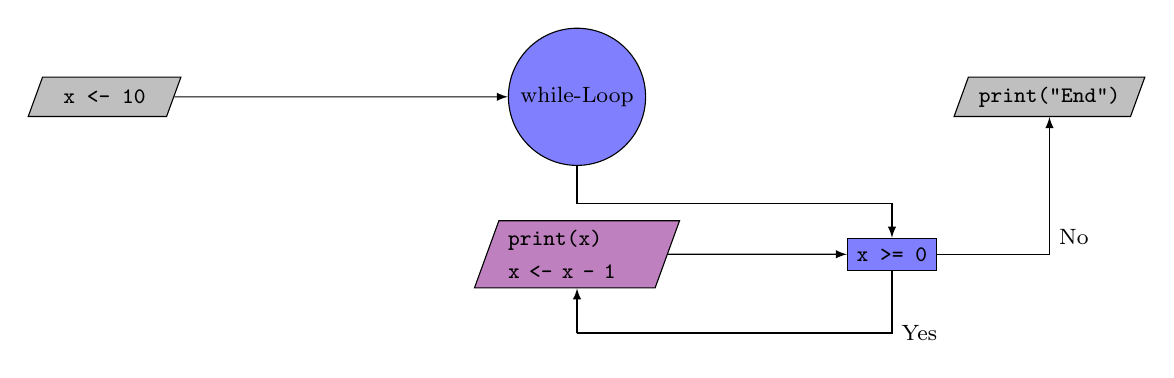
\begin{tikzpicture}
      \node[draw, trapezium, trapezium left angle=70, trapezium right angle=-70, minimum height=0.5cm, fill=gray!50!white] (n0) {\footnotesize \verb+x <- 10+};
      \node[draw, trapezium, trapezium left angle=70, trapezium right angle=-70, right of=n0, node distance=12cm, minimum height=0.5cm, fill=gray!50!white] (nx) {\footnotesize \verb+print("End")+};
      \coordinate[below of=n0, node distance=2cm] (aux1);
      \coordinate[below of=nx, node distance=2cm] (aux2);
      \node[draw, circle, right of=n0, node distance=6cm, fill=blue!50!white] (n1) { \footnotesize while-\newline\footnotesize Loop};
      \node[draw, trapezium, trapezium left angle=70, trapezium right angle=-70, below of=n1, node distance=2cm, minimum height=0.5cm,fill=violet!50!white,text width=1.75cm] (n3) { \footnotesize \verb+print(x)+\\\footnotesize \verb+x <- x - 1+};
      \node[rectangle, draw, right of=n3, node distance=4cm, fill=blue!50!white] (n5) {\footnotesize \verb+x >= 0+};
      \draw[->] (n0) to (n1);
      \coordinate[below of=n1, node distance=1.35cm] (aux4);
      \coordinate[below of=n3, node distance=1cm] (aux5);
      \draw[->] (n1.south) -- (aux4) -| (n5.north);
      \draw[->] (n3) to (n5);
      \draw[->] (n5) |- node[anchor=west]{\footnotesize Yes} (aux5) -| (n3);
      \draw[->] (n5.east) -| node[anchor=south west]{\footnotesize No} (nx.south);
    \end{tikzpicture}
\end{frame}

\begin{frame}[fragile]{Example while-Loop}
  This example demonstrates the while-loop. The condition here is \verb+x >= 0+.\bigskip\\
  \begin{centering}
  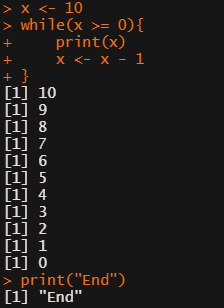
\includegraphics[scale=0.7]{while1.png}
  \end{centering}
\end{frame}

\subsection*{Remarks to for- and while-Loops}

\begin{frame}[fragile]{Remarks to for- and while-Loops}
  \begin{itemize}
    \item The brackets \verb+{+ und \verb+}+ are essential!
    \item Beware of infinite loops!
    \item Any for-loop can be converted into a while loop and vice versa.
    \item Using \verb+break+ a loop can be terminated
    \item With \verb+next+ an iteration can be skipped without terminating the loop
    \item The \verb+apply+-Family offers a nice alternative to loops
    \end{itemize}
\end{frame}

\subsection*{The Apply-Family}

\begin{frame}[fragile]{Apply-Family}
	The apply-family is a collection of functions in R that allows us to \textit{apply} a function onto several inputs one after another. For example, on all rows (or columns) of a matrix, all elements of a list, etc. The different functions are:
	\begin{itemize}
		\item \verb+apply()+
		\item \verb+lapply()+
		\item \verb+sapply()+
		\item \verb+tapply()+
	\end{itemize}
\end{frame}

\begin{frame}[fragile]{apply()}
	With \verb+apply()+ we are able to \textit{apply} a certain function on all rows or columns of a data frame or a matrix, for example to compute all columnwise sums. The basic form is:
	\begin{itemize}
		\item \verb+apply(data, margin, function)+
	\end{itemize}
	For example:
	\begin{columns}[T]
		\begin{column}{0.5\textwidth}
			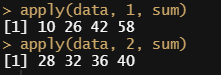
\includegraphics{Apply}
		\end{column}
		\begin{column}{0.4\textwidth}
			\[
			\renewcommand\BAextrarowheight{2pt}
			\begin{blockarray}{*{5}{c}}
				\begin{block}{[*{4}{c}]{c}}
				    1 &2 &3 &4&\textcolor{red}{10}\\
				    5 &6 &7 &8&\textcolor{red}{26}\\
				    9 &10 &11 &12&\textcolor{red}{42}\\
				    13 &14 &15 &16&\textcolor{red}{58}\\
				\end{block}
				\textcolor{red}{28} & \textcolor{red}{32} & \textcolor{red}{36} & \textcolor{red}{40}
			\end{blockarray}
			\]
		\end{column}
	\end{columns}
	
\end{frame}

\begin{frame}[fragile]{lapply()}
	\verb+lapply()+ executes a function on each element of a data frame, a matrix, a vector or a list. The "l" in \verb+lapply()+ is meant for "list" and relates to the fact that \verb+lapply()+ always returns a list.
	\begin{itemize}
		\item \verb+lapply(object, function)+
	\end{itemize}
	For example:\\
	\begin{center}
		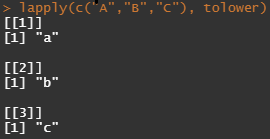
\includegraphics{lapply}
	\end{center}
	
	
\end{frame}

\begin{frame}[fragile]{sapply()}
	\verb+sapply()+ works in the same way as \verb+lapply()+ but always tries to return a nice vector or matrix instead of a list (if possible).
	\begin{itemize}
		\item \verb+sapply(object, function)+
	\end{itemize}
	For example:\\
	\begin{center}
		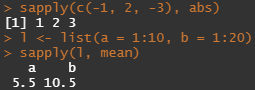
\includegraphics{sapply}
	\end{center}
\end{frame}

\begin{frame}[fragile]{tapply()}
	\verb+tapply()+ allows us to execute functions on different subgroups with respect to some factor variable:
	\begin{itemize}
		\item \verb+tapply(object, index, function)+
	\end{itemize}
	For example:\\
	\begin{center}
		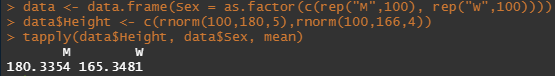
\includegraphics{tapply}
	\end{center}
\end{frame}

\section{Custom Functions}

\begin{frame}[fragile]{Custom Functions}
    So far, we only used pre-defined functions, as for example \verb+t.test+. However, \textsf R allows us to write our own functions. \bigskip \\
Functions have an own datatype that is initalized with the keyword \verb+function()+, followed by a block of code in curly brackets. Within the round parentheses we can define variables freely, which are interpreted as function arguments.
\end{frame}

\begin{frame}[fragile]{Example of a function with one argument}
  For the mathematical function $f(x) = x^2$, the variable $x$ is free (independent). If we want to construct a function in \textsf R that does the same, we do so as follows: \bigskip \\
  \begin{centering}
    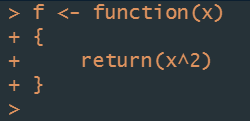
\includegraphics[]{func1.png}
  \end{centering}
\end{frame}

\begin{frame}[fragile]{Remarks to the Definition of Custom Functions}
  \begin{itemize}
    \item Using the brackets \verb+{+ und \verb+}+ is essential!
    \item If you specify function arguments, the user must specify them with each call of the function. \\
An exception is, if we provide default values within the parentheses by initializing the argument directly with \verb+=+
    \item If your function takes more than one argument, you must separate the arguments with a comma 
    \item \textsf R tries to vectorize automatically (if possible), meaning that if a vector or matrix is given as an argument, the function will try to apply the function on each element separately.
    \item If a function is not meant to return anything, then the \verb+return()+ statement can be omitted.
  \end{itemize}
\end{frame}



\end{document}
